\documentclass{article}

\usepackage{amsmath}

\usepackage{graphicx}
\usepackage{subcaption}

\usepackage{float}

\usepackage[margin=2.54cm]{geometry}



\usepackage[style=numeric, sorting=none]{biblatex}
\addbibresource{bib_files/Biblio.bib}

%-------------------------- début du document ---------------------------%


\begin{document}

%----------------------------- page de garde ----------------------------%
\fontsize{12pt}{14pt}\selectfont
\begin{figure}[ht]
\vspace{0.3cm}
    \centering
    \begin{subfigure}[b]{0.2\textwidth}
        
\includegraphics[width=\textwidth]{images/Logo_UM.png}
    \end{subfigure}
    \begin{subfigure}[b]{0.2\textwidth}
        
\includegraphics[width=\textwidth]{images/Logo_FDS.png}
    \end{subfigure}
    \begin{subfigure}[b]{0.2\textwidth}
        
\includegraphics[width=\textwidth]{images/Logo_cea.png}
    \end{subfigure}
\end{figure}

% \floatbarrier

\begin{center}
\vspace{1.2cm}
\LARGE{UNIVERSITÉ DE MONTPELLIER}
	
\vspace{0.8cm}
\LARGE{FACULTÉ DES SCIENCES}

\vspace{0.8cm}
\LARGE{ COMMISSARIAT A L'ENERGIE ATOMIQUE ET AUX ENERGIES ALTERNATIVES}
	
\vspace{1.7cm}	
\Large
\textbf{Report of the Alternance program for the Masters second year in Computational Physics}

\vspace{1.3cm}
\normalsize	{Author :}\\
\vspace{.3cm}
\large{\textbf{Nischal Dhungana}}
	
\vspace{1.3cm}
\normalsize	{Under the supervision of :} \\
\vspace{.3cm}
\large
\textbf{Guillame Freychet}

\vspace{1.3cm}
\textbf{June 2024}
\end{center}

%--------------------------- remerciements ------------------------------%
\newpage
\section*{Acknowledgements}

\medskip


%------------------------------ table des matières ----------------------%
\newpage

\tableofcontents


%----------------------------- outline -----------------------------%

\section{Introduction}

\medskip

The continuous miniaturization of microelectronic components, driven by Moore's Law, 
has led to a significant reduction in transistor size and increased chip complexity.
This rapid advancement has presented new challenges in the field of metrology, the science of measurement.
Existing metrology techniques, such as Optical Critical Dimension (OCD) and Critical Dimension Scanning 
Electron Microscope (CDSEM), are reaching their limits in terms of resolution and accuracy as feature sizes
shrink to the nanometer scale.


\begin{figure}[h]
    \centering
    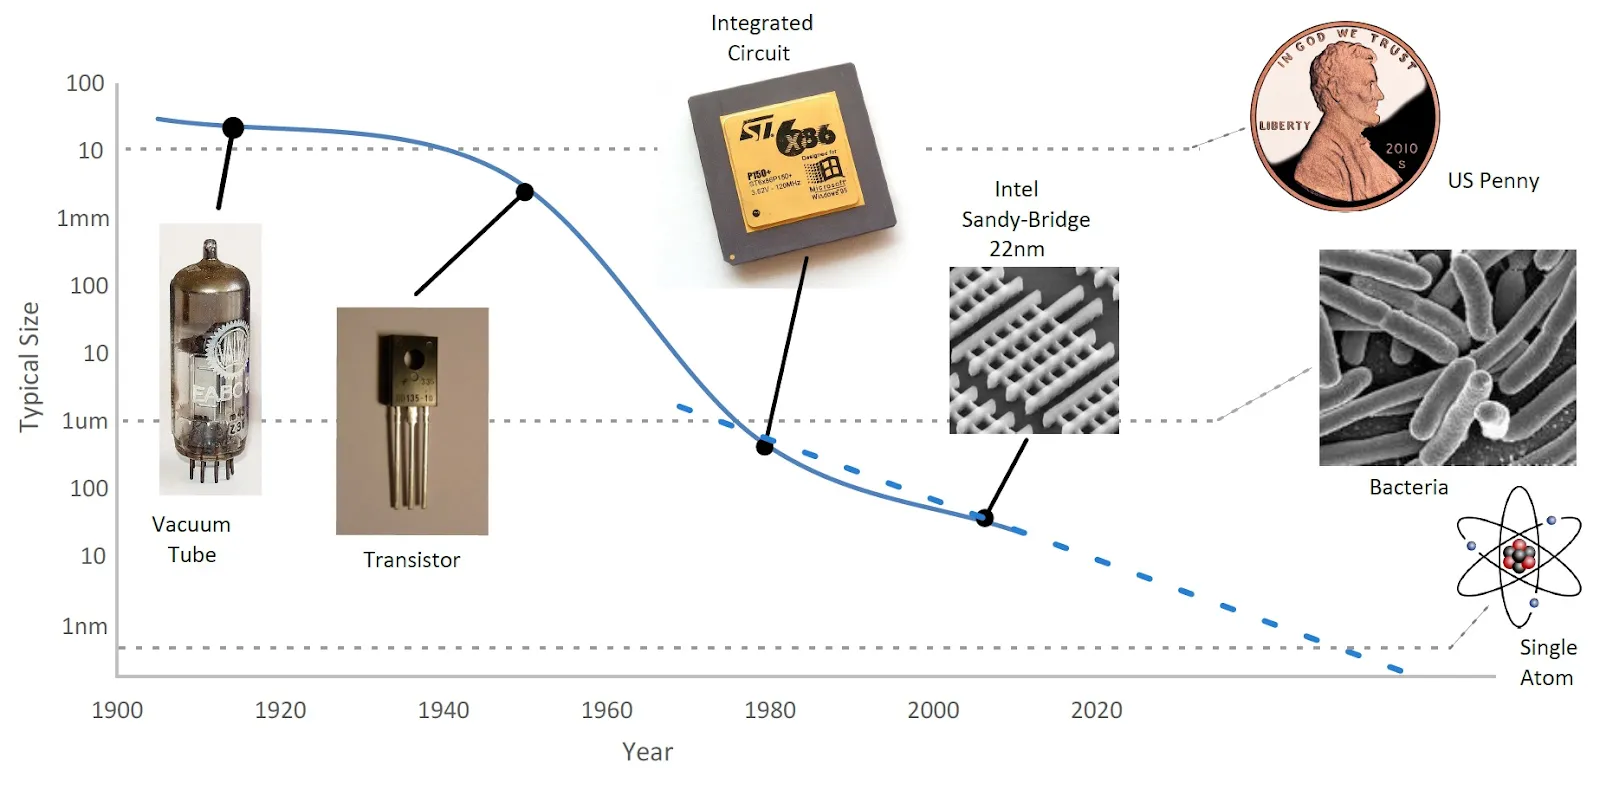
\includegraphics[width=0.8\textwidth]{images/moore's_law.png}
    \caption{Evolution of microelectronics and the need for advanced metrology techniques \cite{moore_law}.}
    \label{fig:evolution_microelectronics}
\end{figure}

\FloatBarrier

To address these challenges, a new metrology technique called Critical Dimension Small Angle X-ray Scattering
(CDSAXS) is being developed. CDSAXS utilizes short-wavelength X-rays $(\lambda \approx 0.05 - 5 nm)$, to probe the internal structure of
materials, providing high-resolution measurements of critical dimensions (CDs) with greater accuracy than
conventional methods. CEA-Leti, a leading research institute in microelectronics, is actively involved in
the development of CDSAXS technology.

\medskip

This work-study project focused on the development of a coherent software for the fit and analysis of CDSAXS
data. The software aims to streamline the data processing workflow and enhance the accuracy of CD measurements.
The project involved a comprehensive understanding of CDSAXS theory, data collection procedures, and fitting
algorithms.

\medskip

The report begins with an overview of the context of the project, highlighting the evolution of
microelectronics and the need for advanced metrology techniques. It then delves into the CDSAXS technique, 
explaining the principles, data collection, fitting, and analysis. Then the subsequent
section describes the software development process, outlining the software's functionalities and design. Finally, the report concludes with a summary of the project's achievements and
outlines potential future directions.

\section{Context}
\subsection{Work environment}
\subsection{Project description}
\subsection{Objectives}


\section{CD-SAXS}
\subsection{Introduction}
\subsection{Theoretical background}
\subsection{Experimental setup}
\subsection{Fitting Algorithm}
\subsection{Analysis of the reconstructed structure}

\section{CD-SAXS Python Application}
\subsection{Introduction}
\subsection{Conception}
\subsection{Simulation Models}
\subsection{On the fly uncertainity estimation}
\subsection{Future Prospects}

\newpage
%generate the bibliography
\printbibliography

\end{document}
